 \chapter{Eventmanagement}
\section{Einführung}
Events beziehungsweise Veranstaltungen sind in den letzten Jahren zu einem der bedeutendsten Marketinginstrumenten sowohl für Unternehmen, Organisationen als auch Privatpersonen aufgestiegen.
Sie ermöglichen und fördern den Aufbau einer starken, persönlichen und emotionalen Beziehung zwischen den Veranstaltern und der dazugehörigen Kundenzielgruppe, was insgesamt zu einer besseren und dauerhafteren Kundenbindung führt.
Ebenso bilden diese real Events einen kreativen Gegenpol zur voranschreitenden Digitalisierung, was durch die vermehrten virtuellen Konversationen und Begegnungen mit anderen Mitmenschen, Arbeitskollegen oder Stakeholdern von jedem einzelnen wahrgenommen werden kann.\autocite[Vgl.][]{Eventmanagementstudieren.de.o.J.}

Mit der globalen Ausbreitung des Covid-19 Virus mussten allerdings die meisten, wenn nicht sogar alle Events abgesagt oder auf unbestimmte Zeit verschoben werden, wie beispielsweise die Fußball Europameisterschaft 2020 oder auch die weltweit wichtigste sicherheitspolitische Konferenz, welche jährlich Anfang des Jahres in München stattfindet. 
Nur die allerwenigsten Veranstaltungen sind durch ein virtuell stattfindendes Event ersetzt worden, was auf die Notwendigkeit dieser einzelnen Veranstaltungen zurückzuführen ist, wie unteranderem der G7-Gipfel.\autocites[Vgl.][]{Tagesschau.o.J.}[Vgl.][]{Nahar.o.J.}[Vgl.][]{ZeitOnline.o.J.}

Das Eventmanagement beinhaltet alle notwendigen Aktivitäten für die erfolgreiche Durchführung eines Events.
Es übernimmt also die Aufgaben der Zielsetzung, operativen Planung und Durchführung in einem vorgegebenen Rahmen.
Im Eventmanagement steht stets der Kunde im Mittelpunkt, weshalb dieses stark von subjektiven sowie psychologischen Aspekten geprägt ist.\autocite[Vgl.][1]{Holzbaur.2002}

\section{Grundlagen des Events}
\subsection{Begrifflichkeit}
Der Begriff \enquote{Event} hat seinen Ursprung im englischen Sprachraum und wird mit \enquote{Ereignis} oder auch \enquote{Veranstaltung} übersetzt.
Aufgrund der stark subjektiven Wahrnehmung von Events gibt es in der Theorie und Praxis keine einheitliche und genaue Definition.
Dennoch kann ein Event durch folgende zentrale Charakteristiken beschrieben werden, welche als Defintion des Begriffs Event in dieser Arbeit dienen: 

\begin{itemize}
    \item Erinnerungswert
    \item Einzigartig- und Einmaligkeit
    \item Aktivierung der Besucher, Positivität
    \item Planung, Organisation und Inszenierung
    \item erlebnisorientierten Ereignis
\end{itemize}\autocite[Vgl.][S. 23 ff.]{Eisermann.2014} 

\subsection{Klassifizierung}
Mit diesem allgemeinen Verständnis von Events soll nun die mögliche Kategorisierung von Events dargelegt werden. 

\begin{table}[!h]
    \centering
    \begin{tabular}{l|l}
        \textbf{Event-Cluster}      & \textbf{Beispiel} \\ \hline
        Kultur-Event                & Open-Air-Konzert, Festival, königliche Hochzeit        \\ \hline
        Sport-Event                 & Super-Bowl, Fußball-WM, Olympia   \\ \hline
        ökonomisches Event          & Apple Keynote, Hauptversammlung   \\ \hline
        politisches Event           & G7-, G20-Gipfel, Münchner Sicherheitskonferenz                   \\ \hline
        natürliches Event           & Sonnenfinsternis, Sternschnuppen        
    \end{tabular}%
    \caption{Eventmanagement: Mögliche Aufteilung von Events in sechs verschiedene Cluster.}
    \label{tab:event-cluster}
\end{table}

Eine grundsätzliche Kategorisierung von Events gibt es in der Literatur aufgrund der Subjektivität nicht, weshalb es zahlreiche unterschiedliche und valide Möglihckeiten der Unterteilung gibt.
So ist beispielsweise eine Unterteilung von Veranstaltungen basierend auf ihrer Größe eine gängige Variante.
Der Autor Walter Freyer schlägt in diesem Kontext die drei Eventgrößen Mega-, Medium- und Mikro-Events vor.
Auch das Clustering basierend auf dem Eventanlasses gehört zu den gängisten Unterteilungsmöglichkeiten, wie in \autoref{tab:event-cluster} verdeutlicht.
Des Weiteren besteht die Möglichkeit zwischen kommerziellen und nicht-kommerziellen Events zu differenzieren.\autocite[Vgl.][S. 23 ff.]{Eisermann.2014} 

\subsection{Ziel}\label{subsec:EM_Ziel}
Nachdem die Hauptmerkmale und Klassifizierungen für Events näher betrachtet worden sind, soll nun die Frge beantwortet werden, weshalb Events durchgeführt werden.
Ein Event wird aus einem bestimmten Grund geplant und durchgeführt.
Deshalb sollte zu Beginn das Ziel bzw. der Zweck des Events festgehalten werden und während des gesamten Eventmanagementprozesses im Kopf behalten werden.
Das jeweilige Ziel eines Events kann sehr unterschiedlich ausfallen und kann unter anderem sein:

\begin{itemize}
    \item Finanzieller Effekt
    \item Einfluss auf Personen
    \item Steigerung der Bekanntheit
    \item Akquirierung von Sponsoren und Teilnehmern
\end{itemize}

Von diesen primären Zielen eines Events lassen sich die sekundären Ziele ableiten.
Mögliche sekundären Ziele sind eine hohe Besucherzahl oder auch eine starke Medienpräsenz.
Insgesamt ist jedes Event am Ziel und folglich am Kunden / Besucher orientiert.
Zum Erreichen dieses Ziels wird bei einem Event mit der Emotionalen Ebene gearbeitet, um die Teilnehmer zu erreichen.
Deshalb ist ein Event stark subjektiv.\autocite[Vgl.][S. 6 ff.]{Holzbaur.2002}

\section{Aufgaben des Eventmanagement}
Das Eventmanagement umfasst alle Aufgaben der Planung, Organisation, Überwachung und Steuerung, die bei der Ausführung eines Events notwendig sind.
Grundsätzlich wird ein Event wie ein Projekt geplant und durchgeführt, weshalb wesentliche Prinzipien des Projektmanagements ebenso im Eventmanagement beachtet werden müssen.
Aus diesem Grund soll an dieser Stelle das magische Dreieck des Projektmanagements vorgestellt werden.\autocite[Vgl.][S. 22]{Holzbaur.2002}

\subsection{Magische Dreieck}
Das magische Dreieck, dargestellt in \autoref{fig:EM_magisches_Dreieck}, besteht aus drei Ecken, die die drei Hauptmerkmale des Projekts repräsentieren:

\begin{figure}[H]
    \centering
    \setlength{\fboxsep}{10pt}
    \setlength{\fboxrule}{0.5pt}
    \fbox{
\includegraphics[width=0.65\textwidth]{img/EM_MagischesDreieck.png}}
    \caption[Eventmanagement: magisches Dreieck]{Darstellung des magischen Dreiecks aus dem Projektmanagements. (Quelle: In Anlehnung \autocite[]{Holzbaur.2002})} \label{fig:EM_magisches_Dreieck}
\end{figure}

\textbf{Ergebnis:} 
\\
Das Hauptmerkmal Ergebnis ist im Eventmanagement das Event selbst und stellt das oberste Ziel des Projektes dar.
Wie bereits im \autoref{subsec:EM_Ziel} beschrieben lassen sich über das Primärziel Sekundärziele ableiten.
Beispielsweise ist das Primärziel die Veranstaltung eines Freundschaftsspiels zwischen einem großen und kleinen Fußballclub, um die finanzielle Situation des kleineren Vereins nach der Corona-Pandemie zu stabilisieren.
Neben dem Sportereignis und den finanziellen Einnahmen, ist das Sekundärziel die Vorstellung des im Sommer getätigten Königstransfers.\autocite[Vgl.][S. 143]{Holzbaur.2002}

\textbf{Ressourcen:}
\\
Das Hauptmerkmal Ressourcen beinhaltet die monetären Mittel, die Infrastruktur wie Räumlichkeiten und Parkplätze sowie das Personal und Arbeitszeit.
Die Ressourcen stellen also alle notwenigen Aufwendung während des gesamten Projekts dar.\autocite[Vgl.][S. 143]{Holzbaur.2002}

\textbf{Zeit:}
\\
Das Hauptmerkmal Zeit oder im Eventmanagement Termin bezieht sich primär auf den Zeitpunkt der Ausführung des Events.
Allerdings zählt zu diesem Haupttermin selbstverständlich auch das Einhalten von davor geplanten Terminen, wie unteranderem das rechtzeitige Plakatieren, versenden der Einladungen oder Verkauf von Event-Tickets.
Dies ist darauf zurückzuführen, dass eine Verzögerung in der Organisation sich negativ auf den Veranstatlungstermin auswirken kann, was bei einem Event grundsätzlich inakzeptabel ist.\autocite[Vgl.][S. 143]{Holzbaur.2002}

Auch im Eventmanagement weisen die drei Hauptmerkmale Wechselwirkungen auf.
So muss beispielsweise ein Ausfall von Personal während der Planung und Organisation des Events, das Hauptmerkmal der Zeit oder des Ergebnisses diese Veränderung im Hauptmerkmal der Ressourcen kompensieren. 


\subsection{Projektstruktur}
Mit dem Wissen, dass ein Event wie ein Projekt zu behandeln ist, muss für das erfolgreiche gelingen eines Events sowohl eine organisatorische als auch inhaltliche Struktur aufgebaut werden.

\subsubsection{Organisatorische Struktur}
Die organisatorische Projektstruktur ist meist eine hierarchische Aufteilung in Aufgabenbereiche beziehungsweise Teilprojekte.
Mit dieser Aufteilung werden für die verschiedenen Bereiche Verantwortliche und Ansprechpartner sichergestellt und eine leichtere Kommunikation ist hierdurch gewahrt.
Eine exmeplarische Projektorganisation eines Events kann in \autoref{fig:EM_Aufbauorganisation} betrachtet werden.\autocite[Vgl.][S. 144 f.]{Holzbaur.2002}

\begin{figure}[H]
    \centering
    \setlength{\fboxsep}{10pt}
    \setlength{\fboxrule}{0.5pt}
    \fbox{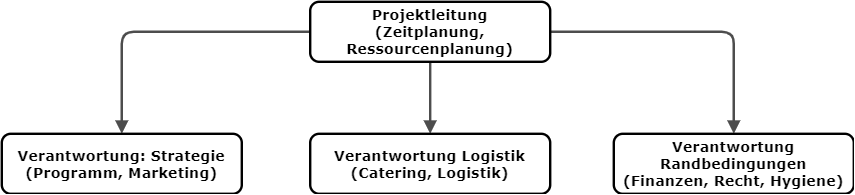
\includegraphics[width=0.8\textwidth]{img/EM_ORG.png}}
    \caption[Eventmanagement: Aufbauorganisation]{Darstellung einer High-Level Aufbauorganisation (Quelle: Eigene Darstellung} \label{fig:EM_Aufbauorganisation}
\end{figure}

\subsubsection{Inhaltliche Struktur}
Die inhaltliche Projektorganisation im Eventmanagement kann über den Projektstrukturplan PSP\autocite[]{projektmanagementdefinitionen.de.o.J.} erreicht werden.
In diesem werden sämtliche Tätigkeiten eines Events aufgenommen.
Tätigkeiten stellen dabei die kleinste Arbeitseinheit dar.
Mehrere Tätigkeiten können wiederum zu einem Arbeitspaket zusammengefasst werden und Arbeitspakete können letztlich zu Teilprojekte aggregiert werden.\autocite[Vgl.][S. 144 f.]{Holzbaur.2002}

Mit Hilfe des Strukturplans erhalten die Verantwortlichen eine bessere Übersicht über die einzelnen Aufgaben und Arbeitspakete.
Außerdem unterstützt der Strukturplan den Projektleiter bei Steuerungs und Controlling spezifischen Aufgaben.\autocite[Vgl.][S. 144 f.]{Holzbaur.2002}

\subsection{Projektplan}
\begin{figure}[H]
    \centering
    \setlength{\fboxsep}{10pt}
    \setlength{\fboxrule}{0.5pt}
    \fbox{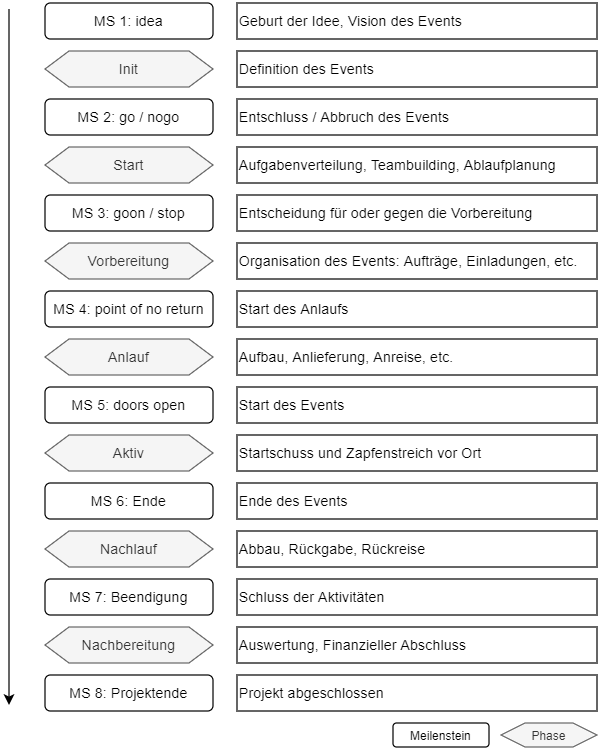
\includegraphics[width=0.85\textwidth]{img/EM_PH_MS.png}}
    \caption[Eventmanagement: Meilensteine und Phase eines Events]{Darstellung der acht Meilensteine und sieben Phasen bei der Veranstaltung eines Events. (Quelle: In Anlehnung \autocite[Vgl.][S. 23]{Holzbaur.2002})} \label{fig:EM_PH_MS}
\end{figure}

Da ein Event auf ein spezifischen Zeitpunkt terminiert ist, der bereits weit im voraus festgelegt wurde, ist es um so wichtiger, diesen Termin ohne Verzögerung eimzuhalten.
Deshalb ist neben einer guten Projektstruktur, ebenso ein gut durchdachter Projekt-/ Eventplan von elementarer Bedeutung.
In \autoref{fig:EM_PH_MS} sind die  Meilensteine sowie Projektphasen für eine erfolgreiche Durchführung eines Events dargestellt.

Die hier aufgezeigten Meilensteine und Phasen stehen in einer engen Beziehung zu einander und können gemeinsam als Grundlage eines Terminplans dienen.
Die Termine und Dauer der jeweiligen Meilensteine und Phasen kann von Event zu Event stark variieren.
Beispielsweise ist die Phase \textit{Aktiv} eines Open-Air-Konzerts nur einige Stunden lang, wohingegen bei einem Musik-Festival diese Phase mehrere Tage dauert.
Grundsätzlich leiten sich die Termine der Meilensteine von der Dauer den jeweiligen Phasen ab.
Der Terminplan kann in einer einfachen Tabelle, Gantt-Diagramm oder ähnlichen Formen abgebildet werden.\autocite[Vgl.][S. 24 ff.]{Holzbaur.2002}

\subsection{Aufgabenbereiche}
Nachdem ein grober Überblick über die Projektstruktur sowie Meilensteine und Eventphasen gegeben worden ist soll nun die verschiedenen Aufgabenbereiche innerhalb eines Events genauer betrachtet werden.
Wie bereits in \autoref{fig:EM_Aufbauorganisation} dargelegt können drei Hauptaufgabenbereiche ausgemacht werden: Strategie, Logistik und Randbedingungen. 

\textit{Strategie:}

Der Aufgabenbereich der Strategie befasst sich mit den Themen Marketing und Programm.
Die Kernaufgabe besteht in der Zieldefinition des Events.
Anschließend kann die Aufgaben der Programmplanung begonnen werden.
Für ein erfolgreiches Entwerfen des Programms ist es notwendig, eine Zielgruppe zu definieren und eine sorgfältige Marktanalyse im Kontext des Eventziels durchzuführen.
Das Eventporgramm der MOBTS 2022 in Mannheim wird in einem folge Kapitel vorgestellt.
Neben der Erstellung des Eventprogramms ist eine weitere wesentliche Aufgabe die Ausarbeitung einer passenden Marketingkampagne.
Beispiele solcher Marketingmaßnahmen sind Werbevideos oder auch Broschüren.
Allerdings müssen je nach Event und Zielgruppe entsprechende Kommunikationswege ausgewählt werden.
Die letzte wesentliche Aufgabe dieses Bereichs besteht in der Suche nach einem möglichen Sponsoring.
Diese Aufgabe kann allerdings je nach Event entfallen.\autocite[Vgl.][S. 168]{Holzbaur.2002}

\textit{Logistik:}

Der Aufgabenbereich der Logistik beinhaltet alle Tätigkeiten, die einen reibungslosen Ablauf eines Events sicherstellen.
Die erste und wichtigste Aufgabe besteht in der Festlegung der Eventlocation.
Diese muss selbstverständlich abhängig des Eventziels und Eventgröße ausgewählt werden.
Des Weiteren organisiert der Aufgabenbereich der Logistik das Catering, die Aufteilung der Räumlichkeiten und für eine eventuelle Bereitstellung von Transportmöglichkeiten wie beispielsweise vom Flughafen zur Eventlocation.
Auch die Müllentsorgung ist Teilaufgabe dieses Aufgabenbereichs und sollte bei der Planung eines Events nicht unberücksichtigt bleiben.\autocite[Vgl.][S. 168 f.]{Holzbaur.2002}

\textit{Randbedingungen:}

Der Aufgabenberiech der Randbedingungen hat drei Hauptaufgaben.
Die erste dieser besteht in der rechtlichen Absicherung.
Beispielsweise können Genehmigung der Stadt notwendig sein, um ein Event an einem Sonntag ausführen zu dürfen.
Die zweite Aufgabe besteht in der Ausarbeitung eines Sicherheits- sowie Gesundheitskonzepts.
Sowohl die Sicherheit als auch Gesundheit muss während eines Events sichergestellt werden.
Durch die Entwicklungen in den letzten Jahren durch verschiedene Attentate aber auch durch die Corona-Pandemie steigt die Wichtigkeit dieser beiden Aspekte.
Durch die Ausarbeitung solcher Konzepte kann in Notsituationen auf diese zurückgegriffen werden, was im Ernstfall Leben retten kann.
Die dritte Hauptaufgabe besteht in der Überwachung der Finanzen und Wirtschaftlichkeit des Events, wie beispielsweise die Buchführung.\autocite[Vgl.][S. 169]{Holzbaur.2002}

Neben diesen drei Aufgabenbereichen kann auch das Projektmanagement als solches gewertet werden.
Allerdings würde eine ausführliche Erläuterung der Aufgaben des Projektmanagements den Rahmen dieser Arbeit sprengen, weshalb auf eine genauere Ausarbeitung verzichtet wird und auf die zahlreiche Literatur, die dieses Thema behandelt, hingewiesen.

\subsection{Zusammenfassung}
Zusammenfassend gibt dieses Kapitel einen Überblick über das Eventmanagement. 
Zunächst ist eine Defintion basierend auf den Charakteristiken gegebn worden und die Möglichkeit der Klassifizierung von Events aufgezeigt. 
Darüberhinaus konnte herausgearbeitet werden, dass das Erreichen des Kunden das oberste Ziel eines Events ist. 
Um sicherzustellen, dass das Event ein Erfolg wird, muss mit Hilfe des Eventmanagements dieses geplant, organisiert, überwacht und gesteuert werden.
Dabei sollten die in diesem Kapitel aufgezeigten Aufgaben berücksichtigt werden.  
Nachdem ein Event wie ein Projekt behandelt wird, sind Erfahrungen im Bereich des Projektmanagements bei der Durchführung eines Events hilfreich.

In den nachfoglenden Kapiteln wird auf die von dual Studierende geplante MOBTS 2022 und dazugehörigen Aktiviäten näher beleuchtet. Dabei soll dieses Kapitel als Grundlage der folge Kapitel dienen. 
